The mixed-initiative controller perceives the human operator and the motion generator as two different agents having the same control rights. The blending mechanism can assess the working conditions' violation and mixes the commands so as the most capable agent has the most control authority at any given moment. An example is when the working conditions include safety rules in the form of collision-free motion, as in this paper. Suppose human inputs compromise the quadrotor's safety. In that case, a violation will be predicted, and the blending will be carried out so that the control authority is mainly given to the motion generator.

Overall, this controller can be seen as an assistive scheme for novice and experienced pilots. Whereas for the former, it allows the pilot to learn to fly a quadrotor without crashing it, for the latter, it introduces some level of disengagement that enables the pilot to fly a quadrotor manually without focusing on avoiding obstacles. 

\begin{figure}[t]
	\centering
	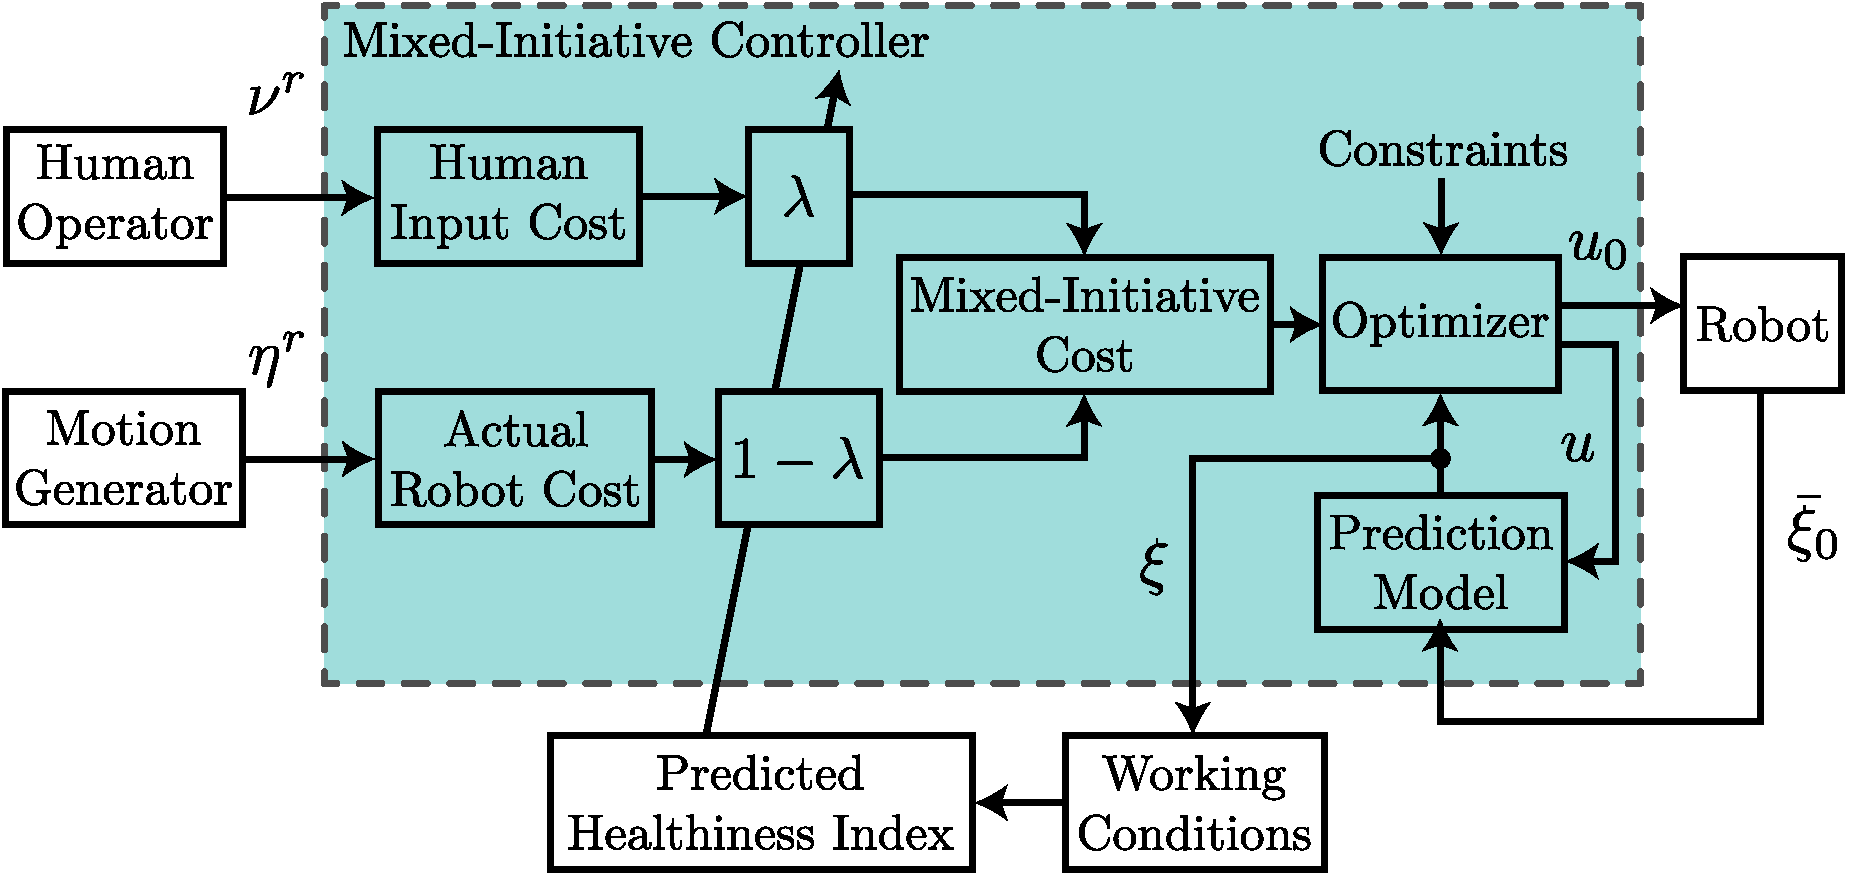
\includegraphics[width=0.49\textwidth]{figures/block_diagram}
	\vspace{-0.6cm}
	\caption{Block diagram summarizing the proposed mixed-initiative control algorithm present in Section \ref{sec:algo_details}.}\label{fig:block_diagram}%
\end{figure}

\subsection{Algorithm overview}
Mixed control is accomplished through a \emph{mixed-initiative NMPC controller} whose cost function -- the \emph{mixed-initiative cost}  -- is a convex combination between the \emph{actual robot cost} and the \emph{human input cost}. The latter is a cost term that penalizes the deviation from the human inputs. The  proposed blending mechanism is a continuous function between 0 and 1, named \emph{predicted healthiness index}, that drives the convex combination. It is computed in this way: when the index tends to 0, the working conditions' violation is too close and, hence, the mixed-initiative cost tends to the actual robot cost. When the index tends to 1, the violation is far enough and, therefore, the mixed-initiative cost tends to the human input cost.

Based on the state solution of the NMPC controller, at each time instant, the predicted healthiness index computes how far the robot is from violating the working conditions within a \emph{virtual horizon} whose length is defined by the designer. It then selects a value between 0 and 1 and blends the commands. The idea is that the closer the index to 0, the more troublesome it will be to keep the system within the working conditions in the next virtual horizon, even if full control is given to the motion generator (and human inputs are heavily ignored from that moment on). Vice-versa, the closer the index to 1, the easier the motion generator's job will be in case it takes full control of the system.  Fig.~\ref{fig:block_diagram} shows a block diagram of the proposed algorithm.